%%%%%%%%%%%%%%%%%%%%%%%%%%%%%%%%%%%%%%%%%
% Simple Sectioned Essay Template
% LaTeX Template
%
% This template has been downloaded from:
% http://www.latextemplates.com
%
% Note:
% The %\lipsum[#] commands throughout this template generate dummy text
% to fill the template out. These commands should all be removed when 
% writing essay content.
%
%%%%%%%%%%%%%%%%%%%%%%%%%%%%%%%%%%%%%%%%%

%----------------------------------------------------------------------------------------
%	PACKAGES AND OTHER DOCUMENT CONFIGURATIONS
%----------------------------------------------------------------------------------------

\documentclass[10pt]{article} % Default font size is 12pt, it can be changed here

\usepackage[spanish]{babel}%Para el español
\usepackage[utf8]{inputenc}%para los acentos
\usepackage{amsmath,amssymb,amsfonts,amsthm}
\usepackage{graphicx}
\usepackage{bbm}
\usepackage{textcomp}
\usepackage{amstext}

\usepackage{geometry} % Required to change the page size to A4
\geometry{a4paper} % Set the page size to be A4 as opposed to the default US Letter

\usepackage{graphicx} % Required for including pictures

\usepackage{float} % Allows putting an [H] in \begin{figure} to specify the exact location of the figure
\usepackage{wrapfig} % Allows in-line images such as the example fish picture

\linespread{1.2} % Line spacing

%\setlength\parindent{0pt} % Uncomment to remove all indentation from paragraphs

\graphicspath{{Imagenes/}} % Specifies the directory where pictures are stored

%\usepackage{tikz}
%%%<
%\usepackage[spanish]{babel}%Para el español
%\usepackage[utf8]{inputenc}
%\usepackage{verbatim}
\usepackage{listings}
%\usepackage{xcolor}


%\usepackage{times}
 
%\definecolor{dkgreen}{rgb}{0,0.6,0}

\lstset{
	language=C,
	literate=%
	{á}{{\'{a}}}1
	{é}{{\'{e}}}1
	{í}{{\'{i}}}1
	{ó}{{\'{o}}}1
	{ú}{{\'{u}}}1
	{ñ}{{\~{n}}}1
	{<}{{$<$}}1
	{>}{{$>$}}1,
	basicstyle=\footnotesize\ttfamily,
	keywordstyle=\bfseries, 
	comment=[l]{\;},%
	breaklines=true,
	prebreak = \raisebox{0ex}[0ex][0ex]{\ensuremath{\hookleftarrow}},
    }

\usepackage{framed}
\usepackage{tabularx,colortbl}
\usepackage{adjustbox}
\usepackage{pdflscape}

\begin{document}


%----------------------------------------------------------------------------------------
%	TITLE PAGE
%----------------------------------------------------------------------------------------

\begin{titlepage}
\newgeometry{left=1.5cm,right=1.5cm}

\newcommand{\HRule}{\rule{\linewidth}{0.5mm}} % Defines a new command for the horizontal lines, change thickness here

\center % Center everything on the page

\textsc{\LARGE Universidad Nacional de Córdoba}\\[1.5cm] % Name of your university/college
\textsc{\Large Informe Trabajo Final}\\[0.5cm] % Major heading such as course name
\textsc{\large Ingeniería de Software}\\[0.5cm] % Minor heading such as course title

\HRule \\[0.4cm]
\Large{ \huge \bfseries Aplicación de las técnicas de Ingeniería de Software sobre un proyecto inconcluso.}\par % Title of your document
\HRule \\[1.5cm]

\begin{minipage}{0.5\textwidth}
\begin{flushleft} \large
\emph{Autores:}\\
Cristian \textsc{Gutierrez} (35.596.222)\\
Esteban \textsc{Morales} (35.104.714)\\
Fabiola \textsc{Campos} (34.243.721)\\
Gianfranco \textsc{Barbiani} (36.372.693)\\
\end{flushleft}
\end{minipage}
~
\begin{minipage}{0.4\textwidth}
\begin{flushright} \large
\emph{Supervisor:} \\
Ing. Martín \textsc{Miceli}
\end{flushright}
\end{minipage}\\[4cm]

{\large \today}\\[3cm] % Date, change the \today to a set date if you want to be precise

%\includegraphics{Logo}\\[1cm] % Include a department/university logo - this will require the graphicx package

\vfill % Fill the rest of the page with whitespace
\restoregeometry
\end{titlepage}

%----------------------------------------------------------------------------------------
%	TABLE OF CONTENTS
%----------------------------------------------------------------------------------------

\tableofcontents % Include a table of contents

\newpage % Begins the essay on a new page instead of on the same page as the table of contents 

%----------------------------------------------------------------------------------------
%	INTRODUCTION
%----------------------------------------------------------------------------------------

\begin{abstract}
En el presente informe se expone el desarrollo del trabajo final para la cátedra Ingeniería de Software que se cursa en el primer cuatrimestre del cuarto año de la carrera Ingeniería en Computación en la Facultad de Ciencias Exáctas, Físicas y Naturales de la Universidad Nacional de Córdoba, Argentina. 
Este trabajo está basado en el ejemplo del Libro Head First design Patterns en la página 526 a 548 (DJView).
\end{abstract} % Major section

\section{Consignas}
\begin{itemize}
\item Modificar la clase HeartModel para que sólo se pueda crear una instancia (usando el patrón 
Singleton) y extienderla ventana de control del BeatController para “tratar” de generar nuevas 
instancias cada vez que se clickea en el  botton “$>>$”. La ventana de  la BeatBar debería mostrar 
en texto el número de intentos de creación de un nuevo HeartBeat model en el texto donde se 
mostraba la frecuencia cardíaca.

\item Crear un nuevo modelo con su controlador específico que pueda usarse para verse desde la 
vista DJView en la ventana BeatBar. Generar un java main class para poder ejecutar tal 
modificación llamándolo \verb+“My<modelName>TestDrive.java”+ (similar to “HeartTestDrive”). Se 
proveerán puntos adicionales por la originalidad del modelo creado.

\item Generar una vista propia que permita usar su modelo sin modificar el código existente del 
ejemplo pero que permita mostrar los cambios gráficamente y por medio de texto (similar al 
BeatBar que muestra el ritmo con una barra y la frecuencia en texto).  

\item Generar un TestDrive que permita mostrar a los tres modelos trabajando al mismo tiempo (se 
esperarán ver al menos 3 ventanas BeatBar con los 3 modelos andando simultáneamente.

\item Modificar la vista BeatBar para que permita cambiar gráficamente en tiempo de ejecución (ej. 
Mediante un dropdown box) el modelo usado (el Beat model, el Nuevo modelo y el Heartbeat 
model). Por favor use para tal implementación el patrón strategy. Generar un TestDrive que 
permita ejecutar tal acción. 

\end{itemize}


\section{Nota de Entrega}
Se entrega junto a este informe:
\begin{itemize}
\item El código fuente del proyecto de software.
\item Los modelos UML en formato imagen y proyecto de VisualParadigm\circledR.
\item Dos (2) archivos ejecutables: para Windows y Linux.
\item Una guía de instalación y ejecución dentro del Readme.md del Repositorio.
\item La presentación con diapositivas en Reveal.js y su equivalente en PDF.
\end{itemize}

\subsection{Listado de Funcionalidad}
Ver detalle en sección 6. %~\ref{sec:Diseño e Implementación}

\subsection{Pass/Fail Ratio del Sistema (PFR)}
Ver detalle en sección 7.%~\{sec:Pruebas Unitarias del Sistema}

\subsection{Vínculo a las fuentes del proyecto}
La dirección web del Repositorio del Proyecto es: "\textit{https://github.com/Andresteve07/FinalIngDeSoftware}".

\section{Manejo de Configuraciones}

\subsection{Plan de Manejo de las Configuraciones}
El plan de manejo de las configuraciones trata y controla:
\begin{itemize}
\item La elaboración de código fuente por varios desarrolladores simultáneamente.
\item El seguimiento del estado de las versiones y sus cambios.
\item La conducción de la integración de las partes del software en un solo producto de software.
\end{itemize}
Para la realización de SCM hay diferentes herramientas. Pero herramientas que pretenden ofrecer una solución total al problema a menudo no cumplen con los requisitos técnicos como:
\begin{itemize}
\item Apoyo a diferentes plataformas.
\item Iniciar el proceso de build.
\item Conexión a los bancos de datos existentes.
\item Integración a la organización existente.
\end{itemize}
Por esa razón ofrece una mayor flexibilidad una solución que integre herramientas parciales que sean más fáciles de integrar en el proceso existente.

\subsection{Herramienta de Control de Versiones}
Para el control de versiones del software que se implemento como consigna del siguiente trabajo final se uso la herramienta de versiones distribuidas y manejo de código fuente "Git". Adicionalmente se respaldó el repositorio en "Github" el cual tiene dirección en: "\textit{https://github.com/Andresteve07/FinalIngDeSoftware}"

\subsection{Sobre los Directorios}
El repositorio cuenta con tres (3) directorios:
\begin{itemize}
\item FinalIngSoft: Este directorio es donde se aloja el proyecto de software desarrollado en la IDE "Eclipse KEPLER" en el lenguaje de programación "JAVA".
\item Informes: En este directorio se encuentra el código fuente escrito en \LaTeX del informe para el trabajo final, un archivo de compilación en PDF y un subdirectorio de imágenes utilizadas.
\item Modelos: Este directorio contiene los proyectos que se realizaron para el modelado UML del software implementado mediante el uso de la herramienta de pago "Visual Paradigm\circledR".
\end{itemize}

\subsection{Etiquetado y Nombramiento de Archivos}
Se decidió del siguiente estándar para el etiquetado y nombramiento del archivos para el proyecto de software:
\begin{itemize}
\item Para los archivos de código fuente escritos en JAVA se adhiere a la costumbre de iniciales en mayúsculas sin espacios.
\item Para las etiquetas sobre las versiones del software se usa la plantilla: "\textsc{vX.Y.Z; con X: Major Version, Y:Minor Version, Z:Patches}"
\end{itemize}

\subsection{Plan del Esquema de Ramas}
Como política de branching se optó por UCM (rebase before deliver).

\begin{figure}[H] % Example image
\center{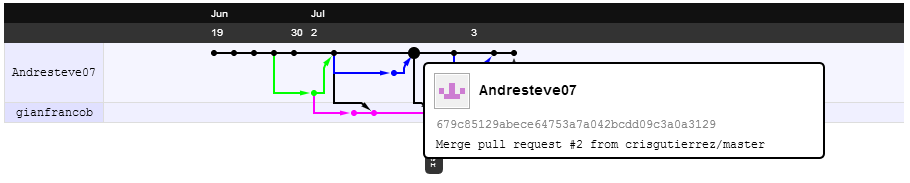
\includegraphics[width=\linewidth]{Branch1}}
\label{fig:Branch1}
\end{figure}

\begin{figure}[H] % Example image
\center{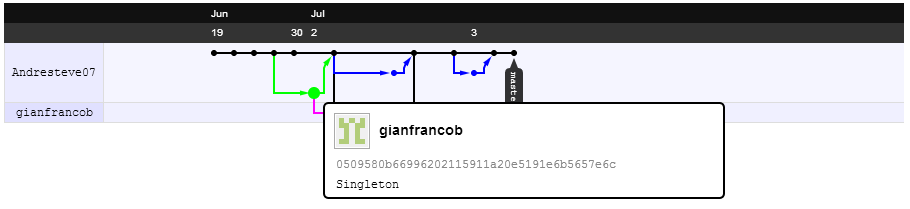
\includegraphics[width=\linewidth]{Branch2}}
\label{fig:Branch2}
\end{figure}

\begin{figure}[H] % Example image
\center{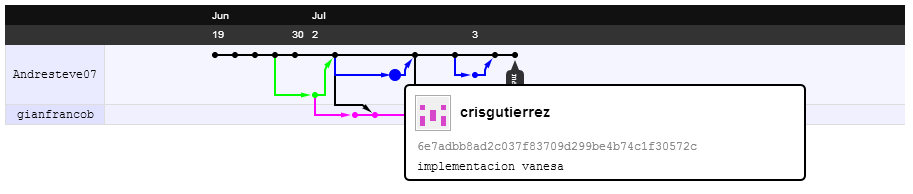
\includegraphics[width=\linewidth]{Branch3}}
\label{fig:Branch3}
\end{figure}

\begin{figure}[H] % Example image
\center{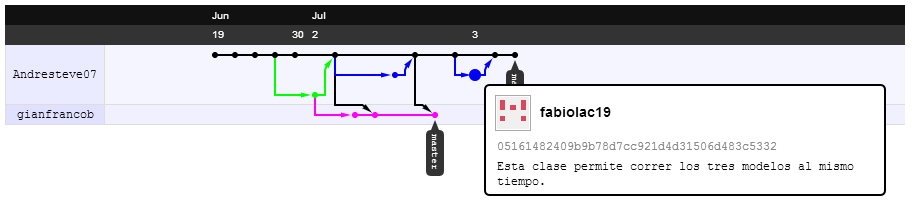
\includegraphics[width=\linewidth]{Branch4}}
\label{fig:Branch4}
\end{figure}

\subsection{Políticas de Marge y de Etiquetado de Progreso.}
Como política de mergeo se decidió que cada desarrollador tenga un fork (o bifurcación, copia) del repositorio original en su cuenta de Github y en su computadora personal, sobre la cual este podrá realizar modificaciones a su conveniencia. Dichos cambios van desde crear branches (ramas) personales hasta etiquetas propias con el objetivo desarrollar la funcionalidad que se le asignó. Una vez terminado su labor, el desarrollador deberá integrar todos los cambios a la rama principal de su fork y recién luego de solucionar los conflictos que hubiere, podrá solicitar un pull request al Configuration Manager (de ahora en más CM) para que la funcionalidad sea integrada el repositorio original.

\subsection{Sobre los Releases}
Forma de entrega de los releases, instrucciones mínimas de instalación y formato de entrega.

\subsubsection{Forma de Entrega}
Una vez conseguida una versión estable el CM generará la etiqueta pertinente respetando el estándar mencionado en la sección 3.4.%~\ref{sec:Etiquetado y Nombramiento de Archivos}. 

\subsubsection{Instrucciones de Instalación}
Dentro del repositorio se encuentra un archivo Readme.txt que explica en forma simple y pocos pasos la instalación y ejecución de un release específico.

\subsubsection{Formato de Entrega}
Se adjuntará al directorio "Releases" dentro del repositorio un archivo con el formato "r\_vX.Y.Z.sh" que es un script de ejecución para un intérprete de bash de Linux.

\subsection{Integrantes}
Listado y forma de contacto de los integrantes del equipo, así como sus roles en la CCB. También incluir periodicidad de las reuniones y miembros obligatorios.
\subsubsection{Roles}


\subsubsection{Sobre las Reuniones}
Las reuniones se acordaron mediante comunicación vía e-mail, y mensajería instantánea. En ellas se encontraron la totalidad de los miembros del equipo.
\begin{itemize}
\item Frecuencia de las reuniones: Encuentros no periódicos de larga duración (XtremePrograming).
\end{itemize}

\subsection{Herramienta de Seguimiento de Errores}
Para el seguimiento de los errores se utilizó el sistema de gestión de issues de provee Github mediante el cual es posible reportar defectos descubiertos, posibles mejoras, detectar código duplicado y realizar preguntas sobre rutinas confusas.

%\subsection{Cualquier otra información relevante}


\section{Requerimientos}
Como parte del REQ\_FUN\_004, denominamos a la nueva clase My<modelName>TestDrive.java como VANESATestDrive; donde VANESA es una sigla que significa: "Visualizador del ANálisis del ESpectro de Audio". A continuación se presentan tres (3) imágenes que exponen lo requerimientos funcionales y no funcionales detectados y su estado al final de la implementación:

\begin{figure}[H] % Example image
\center{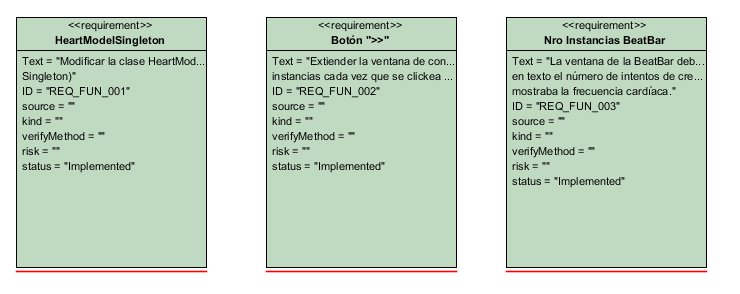
\includegraphics[width=\linewidth]{Diagrama_de_Requerimientos1a}}
\label{fig:Diagrama_de_Requerimientos1a}
\end{figure}

\begin{figure}[H] % Example image
\center{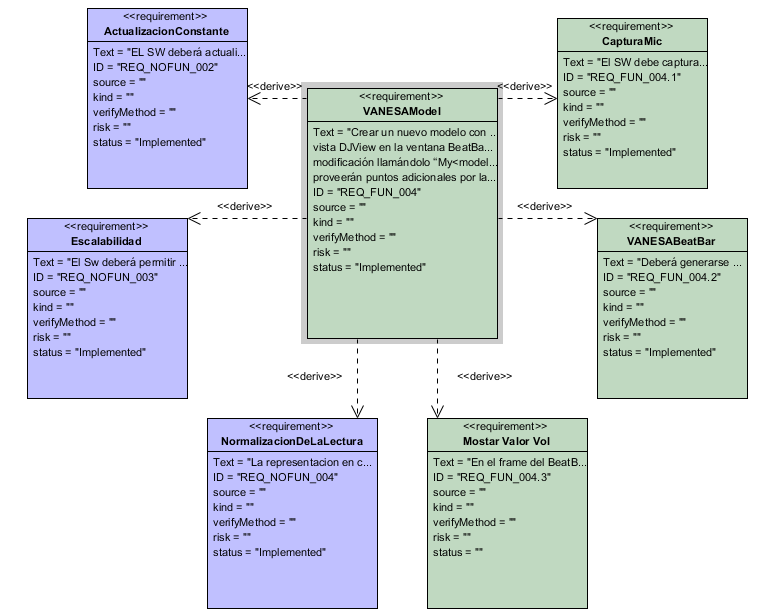
\includegraphics[width=\linewidth]{Diagrama_de_Requerimientos1b}}
\label{fig:Diagrama_de_Requerimientos1b}
\end{figure}

\begin{figure}[H] % Example image
\center{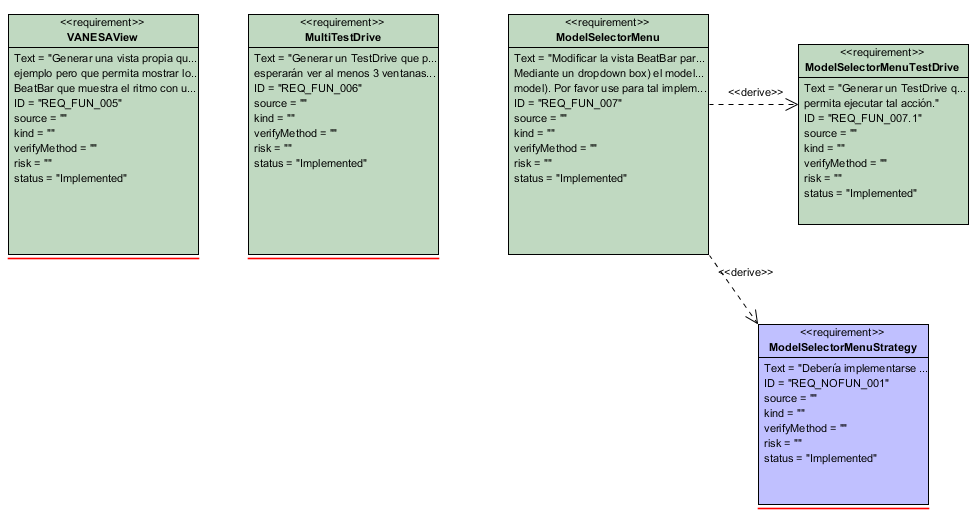
\includegraphics[width=\linewidth]{Diagrama_de_Requerimientos1c}}
\label{fig:Diagrama_de_Requerimientos1c}
\end{figure}

\subsection{Diagramas de Casos de Uso}
En esta sección se muestra el diagrama de casos de usos que surgió de la interpretación preliminar de la consigna:

\begin{figure}[H] % Example image
\center{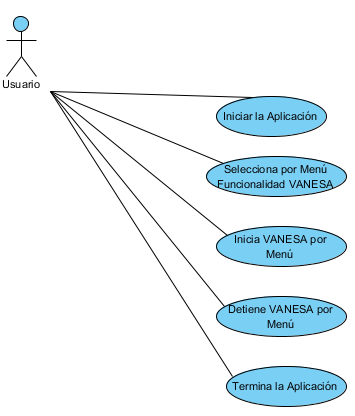
\includegraphics[width=\linewidth]{CasoDeUso}}
\label{fig:CasoDeUso}
\end{figure}

\subsection{Diagramas de Secuencia y Actividad}
Las siguientes imágenes ilustran las representaciones preliminares del diagrama de secuencia y el de actividad para la ejecución del modelo consigna del trabajo:

\begin{figure}[H] % Example image
\center{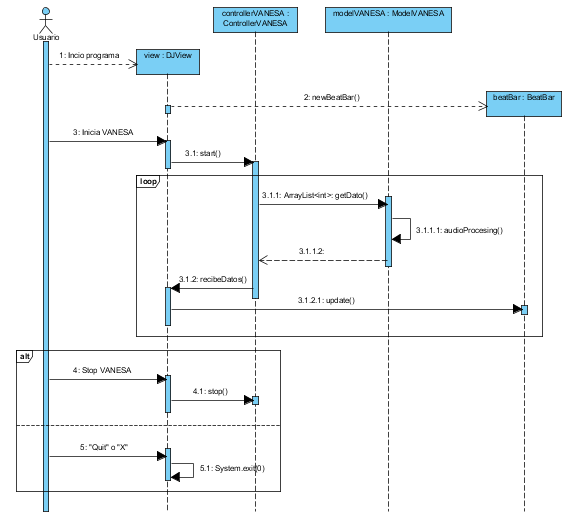
\includegraphics[width=\linewidth]{DiagramaDeSecuencia_Pre}}
\label{fig:DiagramaDeSecuencia_Pre}
\end{figure}

\begin{figure}[H] % Example image
\center{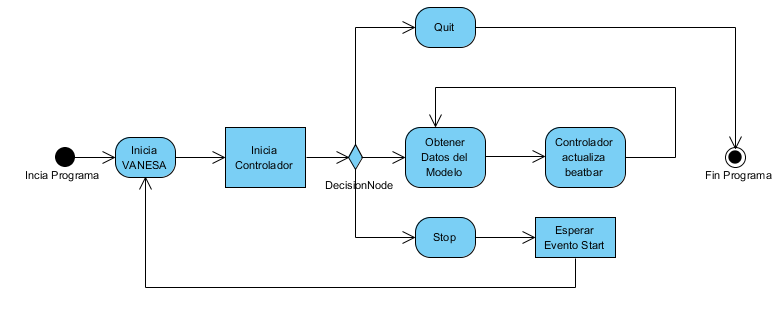
\includegraphics[width=\linewidth]{DiagramaDeActividad_Pre}}
\label{fig:DiagramaDeActividad_Pre}
\end{figure}


%\subsection{Requerimeintos Funcionales del Sistema}

%\subsection{Requerimeintos No Funcionales del Sistema}

%\subsection{Diagrama de Arquitectura Preliminar}

%\subsection{Matriz de Trazabilidad}


\section{Arquitectura}
El software implementa una estricta arquitectura de MVC (Model View Controller). En las siguientes subsecciones se indicará con mayor detalle cuáles partes del código la representan.

\subsection{Gráfico de Arquitectura}
El Patrón de arquitectura MVC es generalmente representada como:

\begin{figure}[H] % Example image
\center{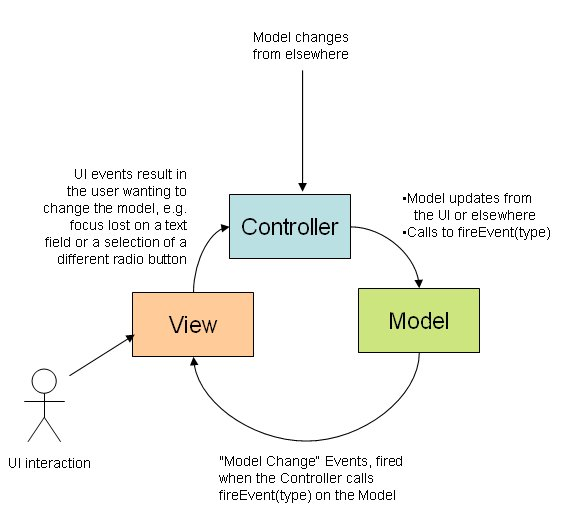
\includegraphics[width=\linewidth]{GenericMVC}}
\label{fig:GenericMVC}
\end{figure}

%\subsection{Componentes vs Interfaces Externas}

\subsection{Patrón de Arquitectura}
El marco de trabajo MVC propuesto originalmente en la década de los 80 como una aproximación al diseño de GU que permitió múltiples presentaciones de un objeto y estilos independientes de interacción de cada una de estas presentaciones.El marco MVC soporta la presentación de los datos de diferentes formas e interacciones independientes con cada una de estas presentaciones. Cuando los datos se modifican a través de una de las presentaciones, el resi de las presentaciones son actualizadas.
Los marcos de trabajo son a menudo instanciaciones de varios patrones. Por ejemplo, el marco MVC incluye el patrón Observer, el patrón Strategy relacionado con la actualización del modelo, el patrón Composite y otros patrones descritos por Gamma y colaboradores(Gammaetal.,1995). 
Las aplicaciones construidas utilizando marcos de trabajo pueden ser las bases para una posterior reutilización a través del concepto de líneas de productos software o familias de aplicaciones. Debido a que estas aplicaciones se construyen utilizando un marco, se simplifica la modificación de miembros de la familia para crear nuevos miembros. 
El problema fundamental con los marcos de trabajo es su complejidad inherente y el tiempo que lleva aprender a utilizarlos. Pueden requerirse varios meses para comprender completamente el marco de trabajo, por lo que es muy probable que, en organizaciones grandes, algunos ingenieros de software se conviertan en especialistas en marcos de trabajo. No hay duda de que ésta es una aproximación efectiva para la reutilización, pero es muy elevado el coste que supone introducirla en los procesos de desarrollo del software.

\subsection{UML de Despliegue}
En esta sección se muestra el diagrama de despliegue que surgió de la interpretación preliminar de la consigna:

\begin{figure}[H] % Example image
\center{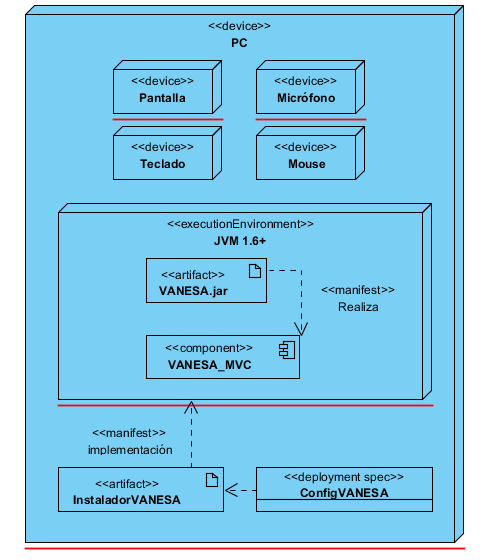
\includegraphics[width=\linewidth]{DiagramaDeDespliegue_Pre}}
\label{fig:DiagramaDeDespliegue_Pre}
\end{figure}

\subsection{UML de Componenetes}
A continuación se presenta una imagen que modela el diagrama de componentes tal y como se detectaron al comienzo de la implementación:

\begin{figure}[H] % Example image
\center{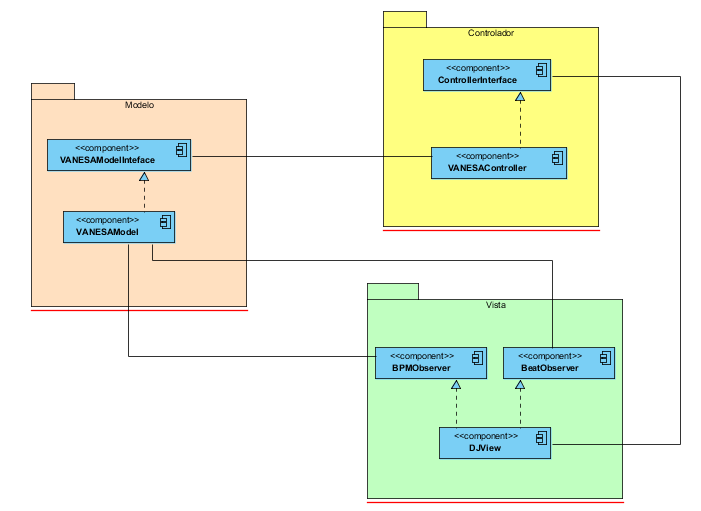
\includegraphics[width=\linewidth]{DiagramaDeComponentes_Pre}}
\label{fig:DiagramaDeComponentes_Pre}
\end{figure}

%\subsection{Diagrama de Contexto}


\section{Diseño e Implementación}

\subsection{Diagrama de Clases}
Con el objetivo de modularizar el código y procurar el encapsulamiento de cada parte, se decidió la implementación de las siguientes clases:
\begin{itemize}
\item Actualizador.java
\item Componente.java
\item FinalConcurrente.java
\item Monitor.java
\item PanelControl.java
\item Proceso.java
\item VentanaPanel.java

\item Controladores
\begin{itemize}
\item /FinalIngSoft/src/Controladores/BeatController.java
\item /FinalIngSoft/src/Controladores/ControllerInterface.java
\item /FinalIngSoft/src/Controladores/HeartController.java
\item /FinalIngSoft/src/Controladores/VANESAController.java

\end{itemize}
\item FinalIngSoft
\begin{itemize}
\item /FinalIngSoft/src/FinalIngSoft/DJTestDrive.java
\item /FinalIngSoft/src/FinalIngSoft/HeartTestDrive.java
\item /FinalIngSoft/src/FinalIngSoft/TestDrive.java
\item /FinalIngSoft/src/FinalIngSoft/VANESATestDrive.java
\item /FinalIngSoft/src/FinalIngSoft/VANESAViewTest.java

\end{itemize}
\item Modelos
\begin{itemize}
\item /FinalIngSoft/src/Modelos/BeatModel.java
\item /FinalIngSoft/src/Modelos/BeatModelInterface.java
\item /FinalIngSoft/src/Modelos/HeartAdapter.java
\item /FinalIngSoft/src/Modelos/HeartModel.java
\item /FinalIngSoft/src/Modelos/HeartModelInterface.java
\item /FinalIngSoft/src/Modelos/VANESAModel.java
\item /FinalIngSoft/src/Modelos/VANESAModelInterface.java

\end{itemize}
\item Testing
\begin{itemize}
\item /FinalIngSoft/src/Testing/VANESAModelTest.java

\end{itemize}
\item Vistas
\begin{itemize}
\item /FinalIngSoft/src/Vistas/BeatBar.java
\item /FinalIngSoft/src/Vistas/BeatObserver.java
\item /FinalIngSoft/src/Vistas/BPMObserver.java
\item /FinalIngSoft/src/Vistas/DJView.java
\item /FinalIngSoft/src/Vistas/VANESAView.java

\end{itemize}


\end{itemize}
Se muestra a continuación el diagrama de clases y luego se desarrollará una breve descripción de las nuevas clases e interfaces implementadas y se detallarán sus métodos más relevantes.
\textit{Imagen demasiado grande para el tamaño de la hoja. Por favor ver "ReverseEngineeringFinalIngSoft\_FINAL.jpg" en el directorio de Imagenes.}

\subsection{VANESAController.java}
Esta clase está encargada de tomar los datos de la View, (de acuerdo a la estrategia MVC), los procesa y con ellos ejecuta funciones del VANESAModel, logrando así la interacción desde el View, pasando por el Controller hasta el Model.

\subsection{TestDrive.java}
Esta clase fue implementada para poder satisfacer el REQ\_FUN\_006, denominado "MultiTestDrive". Su objetivo, es ejecutar y mostrar simultaneamente los tres (3) modelos que posee el proyecto de software.

\subsection{VANESATestDrive.java}
Esta clase crea un modelo del tipo VANESAModel, el cual luego asocia a un controlador específico (VANESAController), y con los cuales mostrará las vistas correspondientes solicitadas.

\subsection{VANESAModel.java}
Esta clase es un hilo que representa el comportamiento descrito por el REQ\_FUN\_004 y sus requerimientos derivados. Sus clases mas importantes son:
\begin{itemize}
\item calculateRMSLevel : int: Calcula y devuelva el valor eficaz de un vector del tipo byte. 
\item getAudioFormat : AudioFormat: Define la frecuencia de muestreo, el tamaño en bits del vector, el número de canales y otras variables y devuelve un nuevo objeto AudioFormat con el cual se realizará la captura de audio del micrófono.
\item run : void: Lee la información de audio de la línea de entrada del buffer. Luego se calcula el valor RMS del arreglo de bytes y con él genera una lectura que representa el volumen de la entrada por micrófono. Finalmente se notifica a todos los observadores. Cabe aclarar que al momento de notificar al BeatBar, este se hace cada un período mayor cuanto menor sea el volumen leído.
\end{itemize}

\subsection{VANESAModelTest.java}
El comportamiento de esta clase sera detallado en la sección 7. %~\ref{sec:Pruebas Unitarias del Sistema}.

\subsection{DJView.java}
Es una clase que se encontraba ya implementada por el código fuente original. Sin embargo, se le realizaron las siguientes modificaciones a fin de satisfacer los requerimientos pertinentes:
\begin{itemize}
\item Se creó el método "setModel", el cual es el encargado de determinar qué modelo se mostrará por la vista. Para hacerlo eficientemente, primeramente remueve los observadores antiguos, refresca el modelo actual al deseado, y finalmente vuelve a registrar los observadores.
\item Se modificó la función "createView" para que crear un menú nuevo (con sus correspondientes items)dentro del frame del BeatBar, así con el permitir seleccionar entre los distintos modelos.
\end{itemize}

\subsection{VANESAView.java}
Es la clase encargada de crear una vista para representar el modelo VANESAModel. Sus funciones son:
\begin{itemize}
\item VANESAView (constructor): Registra los observadores (BeatObserver y BPMObserver) al modelo VANESAModel. A continuación crea una barra de progreso (jp : JProgressBar) a fin de con ella representar gráficamente el nivel de volumen leído por el micrófono.
\item (@Override) updateBPM : void: Este método refresca la etiqueta que muestra el nivel de volumen del micrófono.
\item (@Override) updateBeat : void: En esta función, bajo ciertas condiciones, se "pinta" el valor de volumen del micrófono. 
\end{itemize}

\subsection{Diagrama de Sequencia}
A continuación se muestran varios diagramas de secuencia de ejecución del proceso:

\begin{figure}[H] % Example image
\center{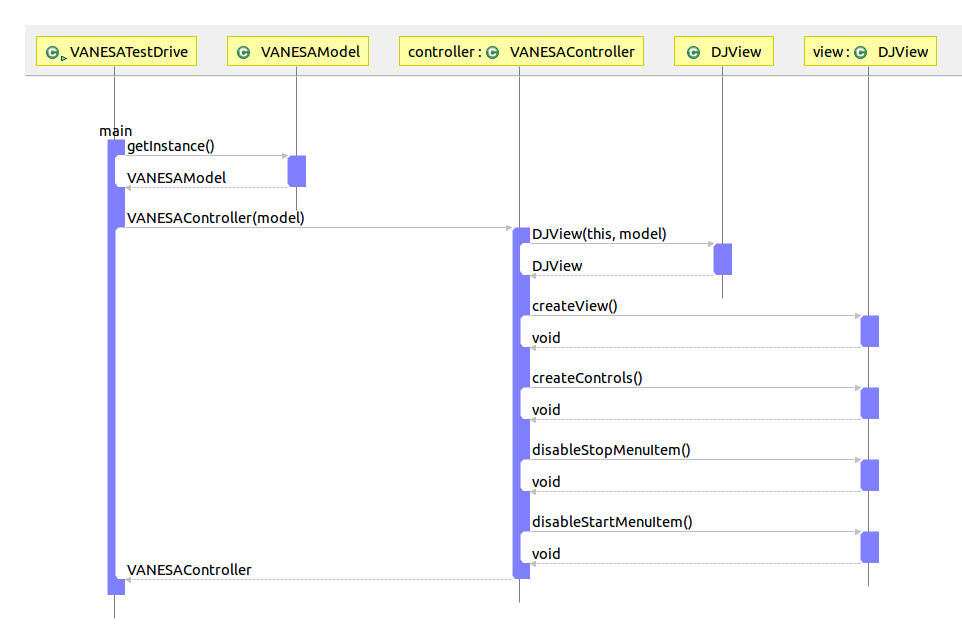
\includegraphics[width=\linewidth]{DiagramaDeSecuencia_Post_a}}
\label{fig:DiagramaDeSecuencia_Post_a}
\end{figure}

\begin{figure}[H] % Example image
\center{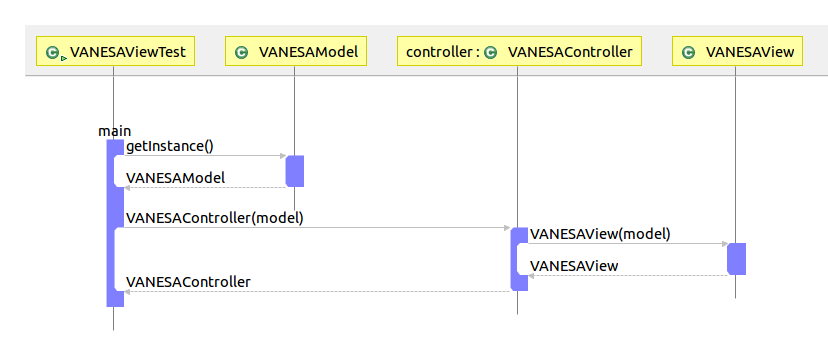
\includegraphics[width=\linewidth]{DiagramaDeSecuencia_Post_b}}
\label{fig:DiagramaDeSecuencia_Post_b}
\end{figure}

\begin{figure}[H] % Example image
\center{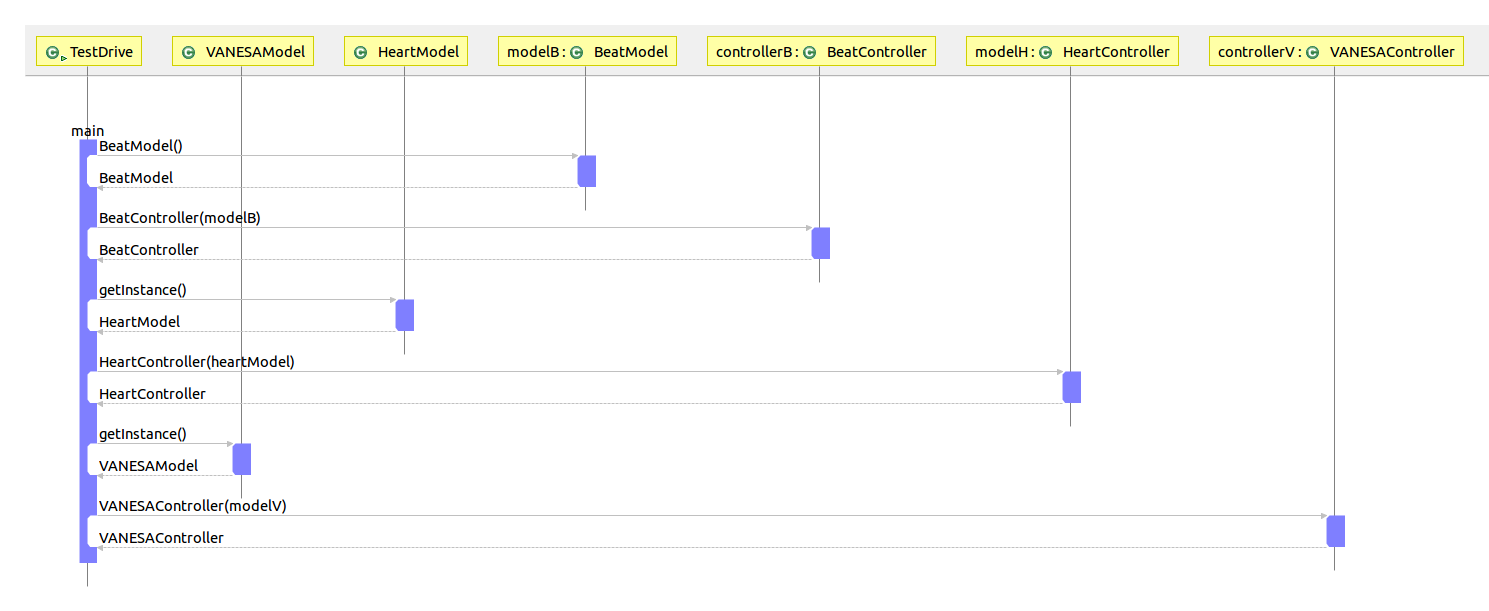
\includegraphics[width=\linewidth]{DiagramaDeSecuencia_Post_c}}
\label{fig:DiagramaDeSecuencia_Post_c}
\end{figure}

%\subsection{Diagrama de Estados}

\subsection{Diagrama de Paquetes}
A continuación se muestran varios diagramas de paquetes que modelan software:

\begin{figure}[H] % Example image
\center{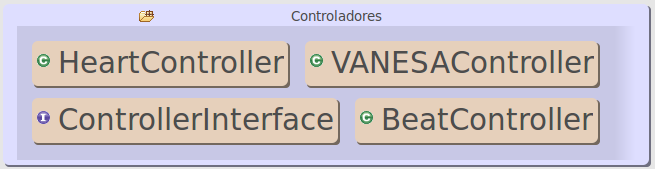
\includegraphics[width=\linewidth]{DiagramaDePaquetes_Post_a}}
\label{fig:DiagramaDePaquetes_Post_a}
\end{figure}

\begin{figure}[H] % Example image
\center{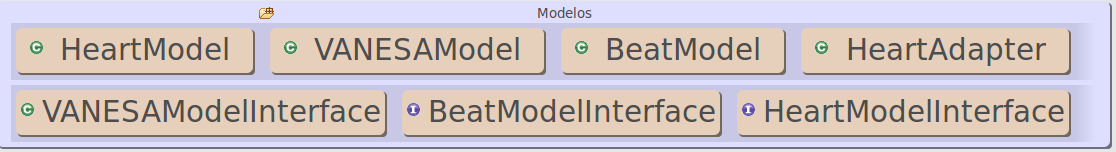
\includegraphics[width=\linewidth]{DiagramaDePaquetes_Post_b}}
\label{fig:DiagramaDePaquetes_Post_b}
\end{figure}

\begin{figure}[H] % Example image
\center{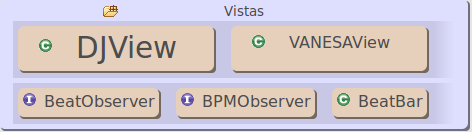
\includegraphics[width=\linewidth]{DiagramaDePaquetes_Post_c}}
\label{fig:DiagramaDePaquetes_Post_c}
\end{figure}

\subsection{Patrón de Diseño adicional implementado}
Se implementó un patrón de diseño Singleton en la clase VANESAModel.

\section{Pruebas Unitarias del Sistema}

\subsection{Pruebas Automáticas}
La clase "VANESAModelTest.java" genera un test unitario para encontrar errores en la clase VANESAModel. Realiza pruebas sobre los métodos "calculateRMSLevel" y "getAudioFormat".

%\subsection{Casos de Prueba del Sistema}
%\subsubsection{Contra los Requerimientos Funcionales del Sistema}
%\subsubsection{Contra los Requerimientos No Funcionales del Sistema}
%\subsection{Casos de Prueba Alternativos}

%\subsection{Smoke/Sanity Tests}

\subsection{Matriz de Trazabilidad Actualizada}
Después de realizar la pruebas unitarias de software y compararlas con los requerimientos del sistema se obtuvo la siguiente matriz de trazabilidad:

\begin{figure}[H] % Example image
\center{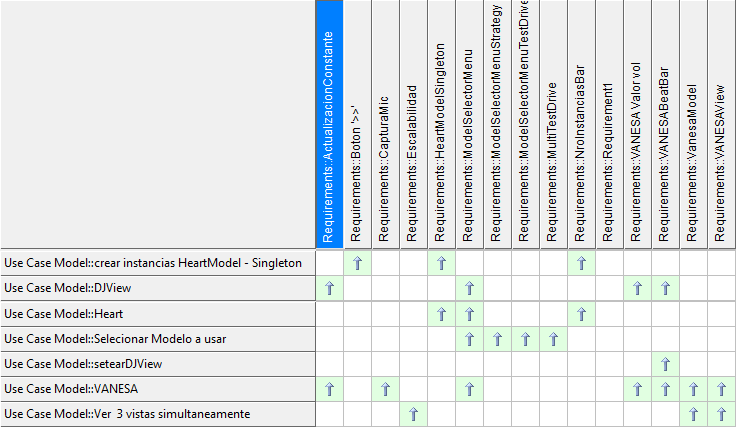
\includegraphics[width=\linewidth]{MatrizDeTrazabilidad}}
\label{fig:MatrizDeTrazabilidad}
\end{figure}

\subsection{Pass/Fail Ratio por tipo de Caso de Prueba}
P/F Ratio = 100\%.

\subsection{Bugs Identificados}

\subsubsection{Corregidos}
Por un lado se identificaron y corrigieron los siguientes bugs:
\begin{itemize}
\item En el DJTestDrive no existía reproducción de sonido. Se corrigió agregando la siguiente linea de código en la posición 85 de la clase BeatModel:\\ 
\verb+sequencer.setMicrosecondPosition(0);+ 
\item En VANESAModel la frecuencia del beatbar no era proporcional al volumen de micrófono, se soluciono haciendo un delay antes de notificar al observador del beatbar, este delay es inversamente proporcional al volumen.
\item En DJView en el beatbar, en el menu para seleccionar el modelo a mostrar, cuando se selecciona un modelo cualquiera, este era mostrado en el view actual pero también se creaba una nueva instancia del mismo. Esto se solucionó en el controlador de cada modelo evaluando si ya existía una instancia del view creada por este controlador, en cuyo caso, de ser así, se trabaja sobre esta y no se crea un nuevo view.
\end{itemize}

\subsubsection{No Corregidos}
Por el otro lado, los siguientes bugs carecen de solución hasta el momento:
\begin{itemize}
\item En VANESAModel el nivel mínimo que toma la lectura del micrófono depende del micrófono, no solucionado.
\item En VANESAView la vista la barra creada es de color naranja, cuando corremos este view junto con DJView el beatbar pasa a ser naranja, no solucionado.
\end{itemize}

\section{Datos Históricos}
\subsection{Cantidad de horas de producción}
\begin{center}
\begin{tabular}{c c c}
\hline\hline %inserts double horizontal lines 
Fecha de Reunión & Duración [Hs]\#1 & Total Horas x Persona [Hs] \\ [0.5ex] % inserts table 
%heading 
\hline % inserts single horizontal line 
Vie 13/06 & 8 & 32 \\ % inserting body of the table 
Mie 25/06 & 6 & 24 \\ 
Sab 28/06 & 7 & 28 \\ 
Lun 30/06 & 6 & 24 \\ 
Mie 02/07 & 12 & 48 \\ 
Jue 03/07 & 14 & 56 \\
Vie 04/07 & 8 & 24 \\ [1ex] % [1ex] adds vertical space 
\hline %inserts single line 
\end{tabular}
\end{center}

\section{Información Adicional}

%----------------------------------------------------------------------------------------
%	CONCLUSION
%----------------------------------------------------------------------------------------

\subsection{Conclusión} % Major section

Implementar la consigna nos permitió aplicar diferentes patrones de diseño de software.
El uso de una herramienta de manejo de la configuraciones nos permitió tener contacto con una experiencia símil profesional de desarrollo de software, así como también aprovechar las ventajas del uso de un sistema automático de versionado. Adicionalmente hicimos uso de un sistema de control colaborativo de revisión y desarrollo de software (Github).
El modelado preliminar del sistema nos ayudó a descubrir nuevo requerimientos, prever futuras fallas del software e inferir patrones de diseño que agilizaron el desarrollo del proyecto.
Una de las partes mas desafiantes del trabajo fue plantear los casos de pruebas para los componentes mas importantes del sistema.
En cuanto a la práctica de la programación, amplió nuestros conocimientos acerca de las librerías que brinda JAVA para el desarrollo de GUI's.
Desafortunadamente resulto muy frustrante no poder cumplir con nuestra voluntad inicial de llevar a cabo el proyecto implementando un modelo de desarrollo ágil (SCRUM), debido a que el tiempo y el esfuerzo dedicado tanto a la planificación como a las otras ceremonias, consumían el poco tiempo que disponíamos para la entrega del proyecto.

%%\lipsum[12-13]

%----------------------------------------------------------------------------------------
%	BIBLIOGRAPHY
%----------------------------------------------------------------------------------------

\begin{thebibliography}{99} % Bibliography - this is intentionally simple in this template

\bibitem[1]{Addison-Wesley}
 \textsc{Sommerville, Ian}
\textit{Software Engineering}
2011, Pearson Education, Inc., publishing as Addison-Wesley

Head First Design Patterns
By Eric Freeman, Elisabeth Robson, Bert Bates, Kathy Sierra
Publisher: 
Released: October 2004

\bibitem[1]{O'Reilly Media}
 \textsc{Eric Freeman}, \textsc{Bert Bates}, \textsc{Kathy Sierra} and \textsc{Elisabeth Robson}
\textit{Head First Design Patterns}
October 2004


\end{thebibliography}

%----------------------------------------------------------------------------------------

\end{document}
